\documentclass[11pt,a4paper]{article}

\usepackage[T1]{fontenc}
\usepackage{cite}
\usepackage{amsmath,amssymb,amsfonts}
\usepackage{graphicx}
\usepackage{booktabs}
\usepackage{array}
\usepackage{url}
\usepackage{xcolor}
\usepackage{float}
\usepackage[section]{placeins}
\usepackage[margin=1in]{geometry}
\usepackage{authblk}
\usepackage{titlesec}
\usepackage{caption}
\usepackage{setspace}

\onehalfspacing
\captionsetup{font=small,labelfont=bf,skip=3pt}
\setlength{\textfloatsep}{8pt plus 2pt minus 2pt}
\setlength{\floatsep}{8pt plus 2pt minus 2pt}
\setlength{\intextsep}{8pt plus 2pt minus 2pt}
\titleformat{\section}{\large\bfseries}{\thesection.}{0.6em}{}
\titleformat{\subsection}{\normalsize\bfseries}{\thesubsection.}{0.6em}{}
\hbadness=10000
\hfuzz=13pt

\title{Comparative US AQI Time Series Forecasting in California with Extreme-Event and Climate-Context Evaluation}
\author{Ta Nguyen Anh Minh \and Trinh Quoc Sang}
\affil{FPT University}
\date{}

\begin{document}
\maketitle

\begin{abstract}
This paper presents a rigorous hourly US AQI forecasting benchmark in California using a merged panel dataset of 181,122 observations from 2018--2025. The panel combines U.S. EPA Air Quality System observations and Open-Meteo supplemental records for Fresno, Los Angeles, and San Jose, with \texttt{target\_aqi} defined as a PM2.5-derived AQI target. Five tabular regressors are evaluated: Linear Ridge, Random Forest, LightGBM, CatBoost, and XGBoost. The experimental design adopts a climate-context-aware temporal split that reserves the extreme 2020 season for validation and uses 2025 as an independent test year. Two operational configurations are assessed: short-term nowcasting with 1--3 hour AQI lags and strict 24-hour-ahead forecasting that hides local AQI information from $t-1$ to $t-23$. LightGBM provides the best benchmark performance among the tested models, achieving an $R^2$ of 0.8691 in the nowcasting setting and 0.4605 at the 24-hour horizon. Feature ablations show that engineered vapor pressure deficit (VPD) and spatial AQI lags have modest standalone effects on global metrics, while the extreme-event analysis reveals distinct temporal clustering during high-pollution episodes without external causal smoke verification.
\end{abstract}

\noindent\textbf{Keywords:} US AQI forecasting, PM2.5, California, time-series regression, climate-context evaluation, vapor pressure deficit, spatial lag, LightGBM, extreme-event analysis.

\section{Introduction}
Air quality forecasting is important for public-health communication, environmental monitoring, and operational warning systems. In California, AQI dynamics are especially challenging because urban emissions, regional meteorology, marine influence, topography, wildfire seasons, and smoke transport can interact over multiple temporal scales. A forecasting system that performs well on ordinary days may still fail during upper-tail pollution episodes, while a model that appears strong under random validation may be overestimated because neighboring time points are highly autocorrelated.

This paper studies comparative US AQI time-series forecasting for California using a reproducible hourly panel. The analysis is designed around two questions. First, how well do common tabular machine-learning models forecast AQI under a near-term autoregressive setting and a stricter 24-hour-ahead setting? Second, how stable are these models under climate-context and extreme-event evaluation, rather than only global test-year metrics?

The contributions are fourfold. First, the paper constructs a California AQI benchmark using harmonized EPA AQS and Open-Meteo records \cite{epa_aqs,epa_aqs_api}. Second, it uses a temporal split that reserves 2020 as an extreme/wildfire-context validation year and 2025 as an independent final test year. Third, it introduces physically interpretable engineered context features, including VPD as an engineered dryness feature and cross-station spatial AQI lags. Fourth, it evaluates the benchmark using leaderboard metrics, scenario slices, ablation testing, and an explicit extreme-event diagnostic. The interpretation is intentionally conservative: engineered physical features are analyzed as contextual signals, not as proven causal drivers of model improvement unless supported by ablation evidence.

\section{Related Work}
Air-quality forecasting has historically used statistical time-series methods such as autoregression and linear regression. These methods are interpretable and often competitive when pollutant persistence is strong, but they may struggle with nonlinear pollutant-meteorology interactions. Modern tabular machine-learning methods provide greater flexibility. Random Forest is a strong bagging-based baseline for nonlinear regression \cite{breiman2001random}, while gradient-boosted decision-tree models such as XGBoost, LightGBM, and CatBoost are widely used for structured environmental data because they can capture threshold effects and heterogeneous feature interactions \cite{chen2016xgboost,ke2017lightgbm,prokhorenkova2018catboost}. Urban air-quality inference work has also emphasized the role of spatial context from nearby monitoring sites \cite{zheng2013uair}.

Evaluation design is equally important. For time-series data, random splitting can leak temporal information because nearby observations share lagged pollutant states, weather regimes, and seasonal context. Time-aware validation is therefore preferred when the goal is operational generalization \cite{bergmeir2018note,roberts2017crossvalidation}. This project follows that principle by separating training, validation, and test periods chronologically, while also using 2020 as a validation year because it contains substantial extreme-AQI context.

\section{Dataset and Exploratory Analysis}
\subsection{Study Area and Data Sources}
The dataset covers Fresno, Los Angeles, and San Jose, combining EPA AQS monitoring records with Open-Meteo supplemental meteorological and AQI-related variables. The modeling target, \texttt{target\_aqi}, is a PM2.5-derived AQI proxy after harmonization and alignment. Current PM2.5 and PM10 proxy variables are excluded from the feature matrix to avoid direct target proxy leakage.

\begin{figure}[H]
    \centering
    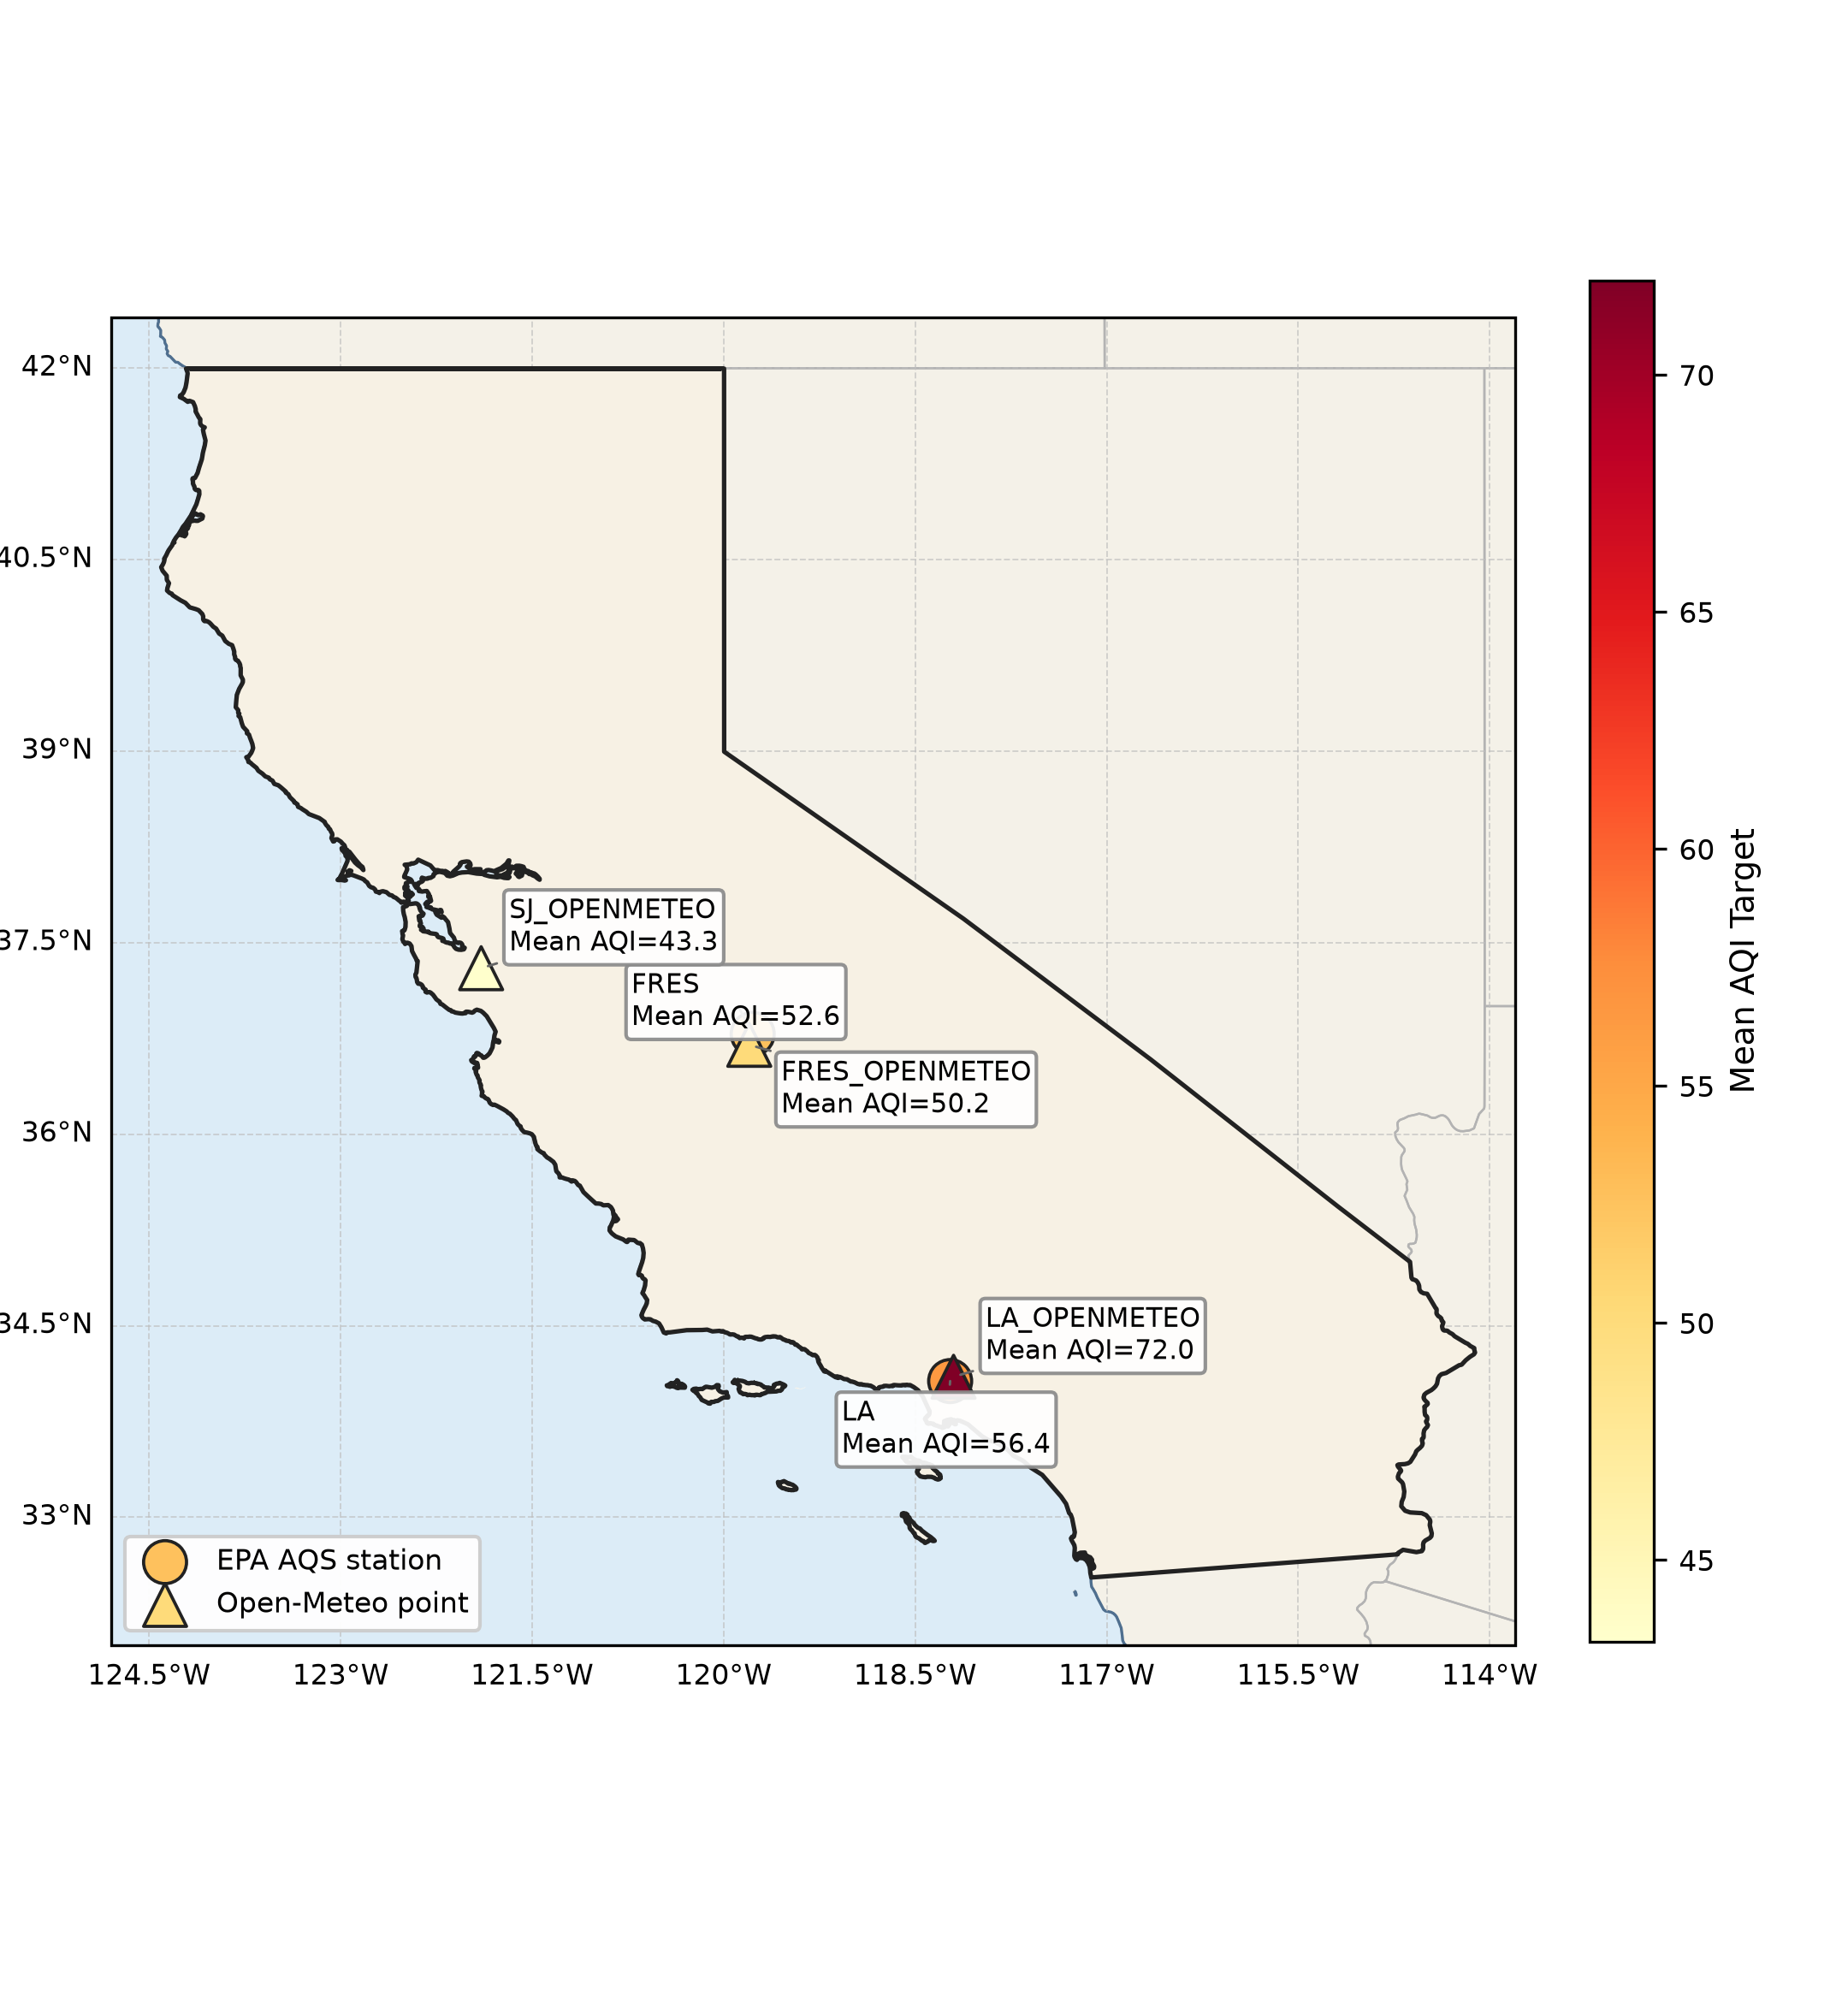
\includegraphics[width=0.58\linewidth]{data/plots/paper_station_map.png}
    \caption{Spatial coverage of the California AQI panel dataset. The figure is included as a static paper asset and is not regenerated by the current figure-generation script.}
    \label{fig:station-map}
\end{figure}
\FloatBarrier

After preprocessing, the model-ready table contains 181,122 hourly records and 21 base columns before scenario-specific lag expansion. The observed target distribution is right-skewed: the mean AQI is approximately 54.79, the median is approximately 54.54, the 95th percentile is 97.21, and the 99th percentile is 151.84. This upper-tail behavior motivates separate scenario and extreme-event evaluation rather than relying only on full-year average errors.

\subsection{Exploratory Correlation Structure}
The exploratory analysis shows that PM2.5 is the strongest direct correlate of the AQI proxy, while meteorological variables provide weaker but meaningful context. Wind speed tends to be negatively associated with AQI, consistent with dispersion effects, although correlation is not evidence of causality. The correlation heatmap is used as a diagnostic overview, not as a feature-selection proof.

\begin{figure}[H]
    \centering
    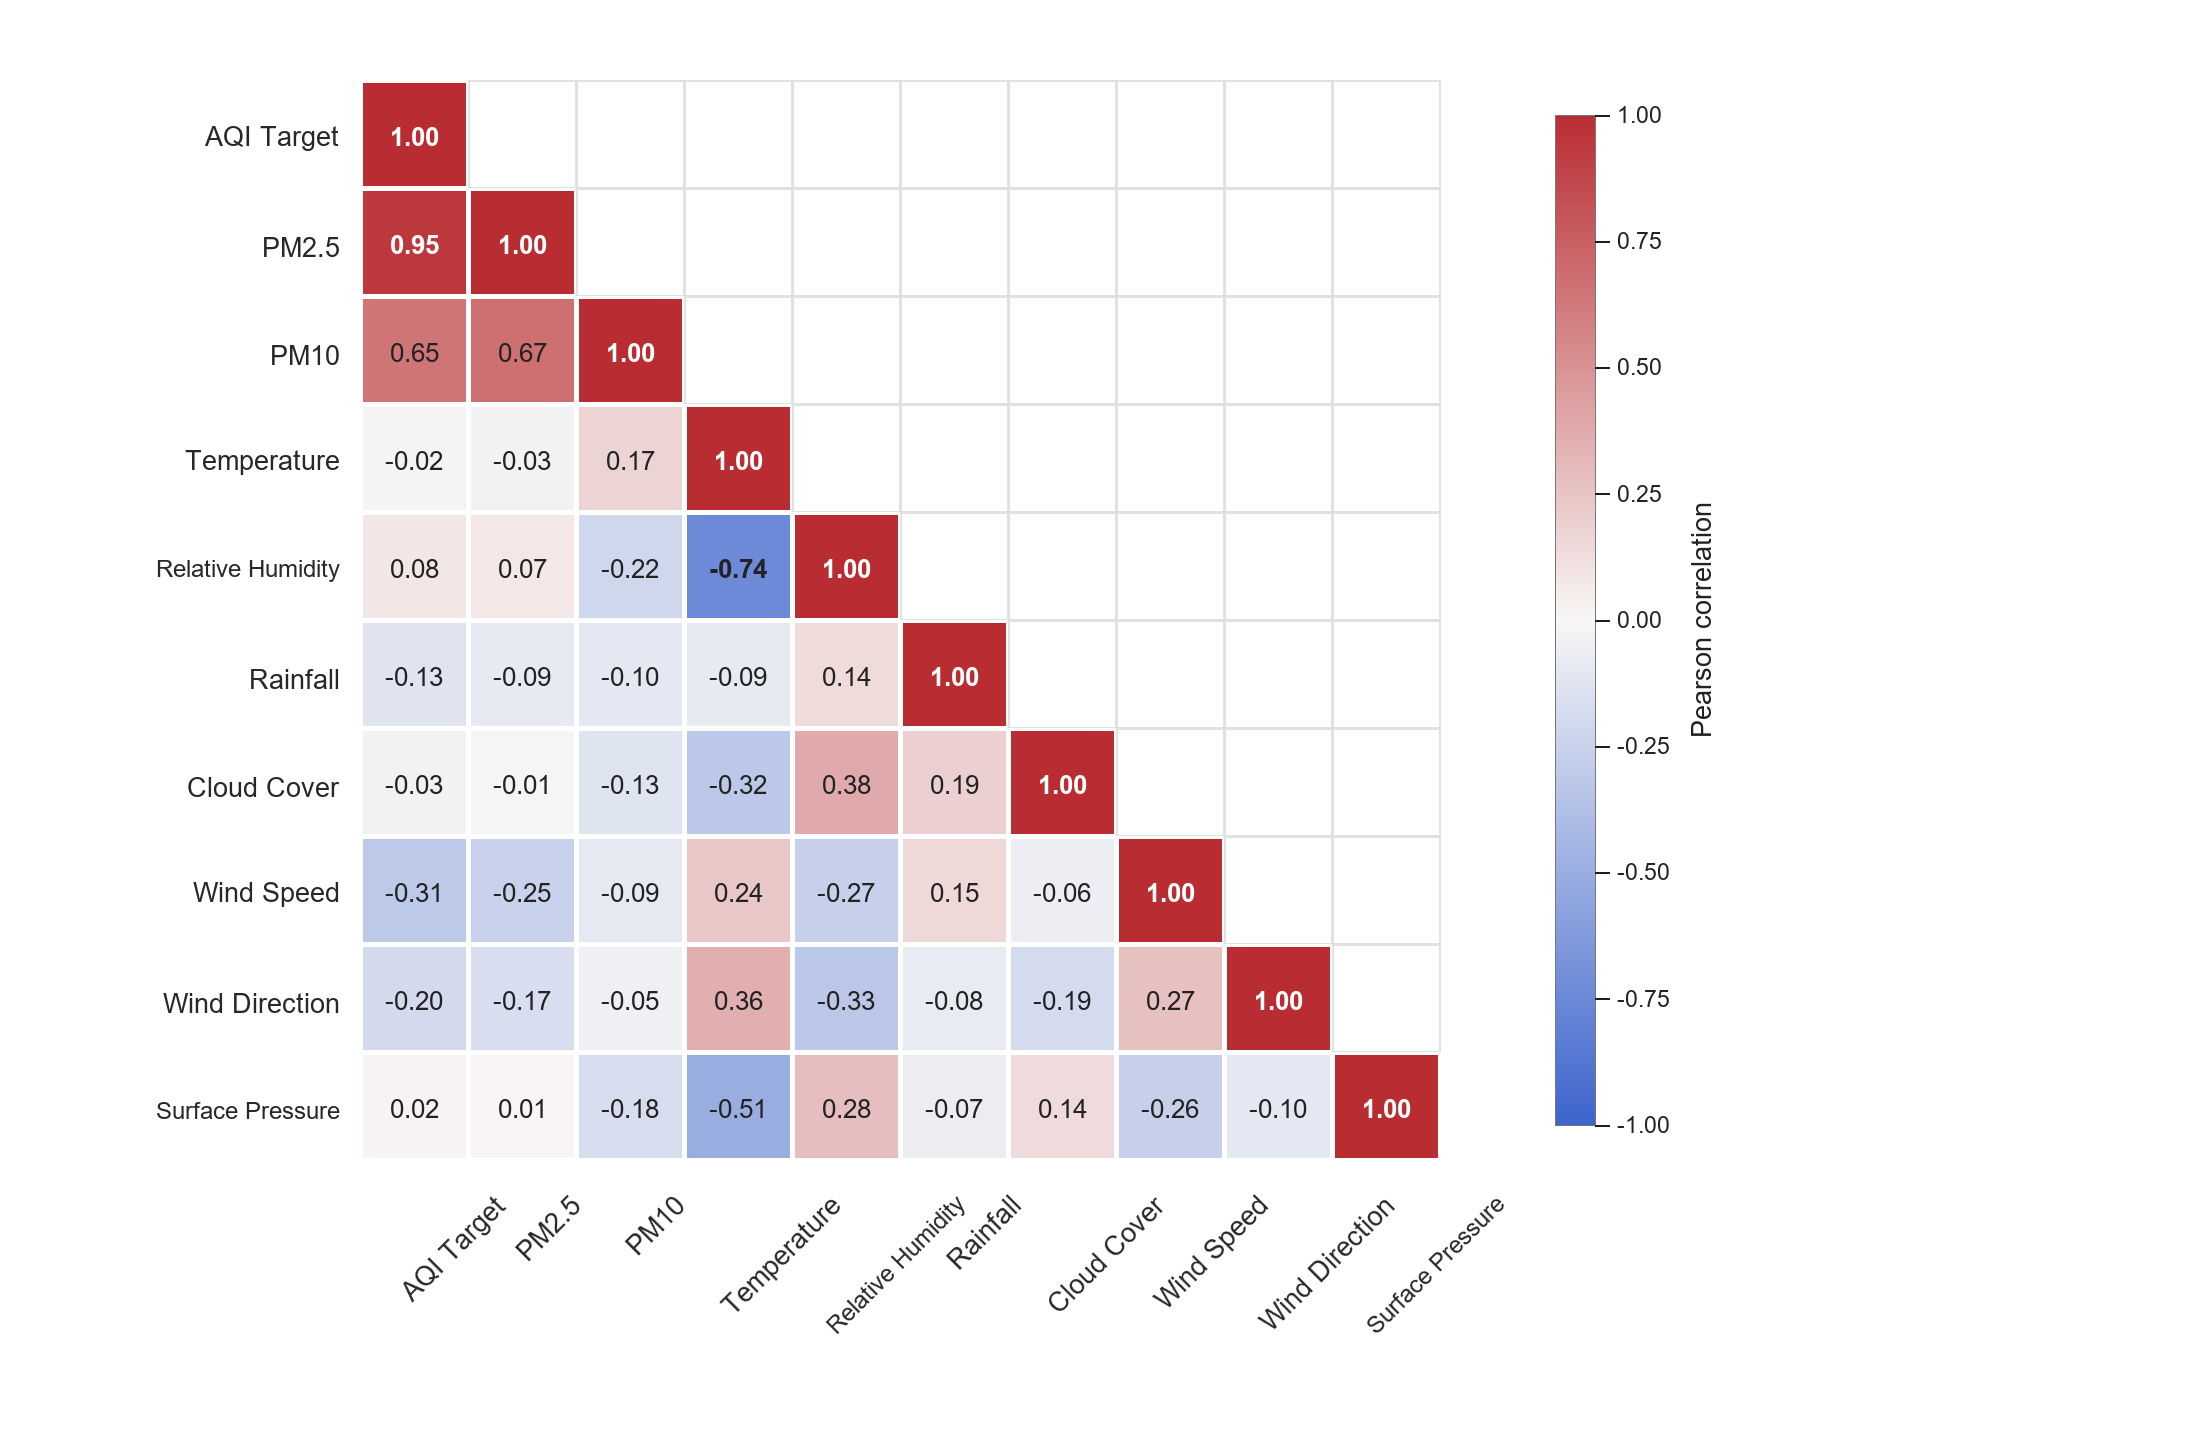
\includegraphics[width=0.82\linewidth]{data/plots/paper_correlation_heatmap_en.png}
    \caption{Pearson correlation heatmap for selected AQI, pollutant, and meteorological variables in the model-ready California panel.}
    \label{fig:correlation-heatmap}
\end{figure}
\FloatBarrier

\section{Feature Engineering}
\subsection{Engineered Dryness Feature: VPD}
Vapor pressure deficit is included as an engineered dryness feature. It summarizes atmospheric moisture demand by comparing saturation vapor pressure with actual vapor pressure, following standard agro-meteorological formulations \cite{allen1998crop}. VPD is also widely used as a physically interpretable indicator of atmospheric dryness and plant-water stress \cite{grossiord2020plant}. In this paper, VPD is not presented as a feature that is proven to improve model accuracy by itself; instead, it is treated as a physically interpretable dryness context variable that can help describe seasonal and meteorological conditions.

Given temperature $T$ in degrees Celsius and relative humidity $\mathrm{RH}$ in percent, saturation vapor pressure is computed as
\begin{equation}
    e_s(T)=0.6108 \exp\left(\frac{17.27T}{T+237.3}\right).
    \label{eq:saturation-vapor-pressure}
\end{equation}
Actual vapor pressure is computed as
\begin{equation}
    e_a(T,\mathrm{RH})=\frac{\mathrm{RH}}{100}e_s(T).
    \label{eq:actual-vapor-pressure}
\end{equation}
The engineered VPD feature is then
\begin{equation}
    \mathrm{VPD}=\max\left(e_s(T)-e_a(T,\mathrm{RH}),0\right).
    \label{eq:vpd}
\end{equation}

The exploratory notebook recomputes VPD from the model-ready meteorological variables and produces a monthly diagnostic plot. This diagnostic is used to verify that the engineered dryness signal follows plausible seasonal structure before it is used in the forecasting feature set.

\begin{figure}[H]
    \centering
    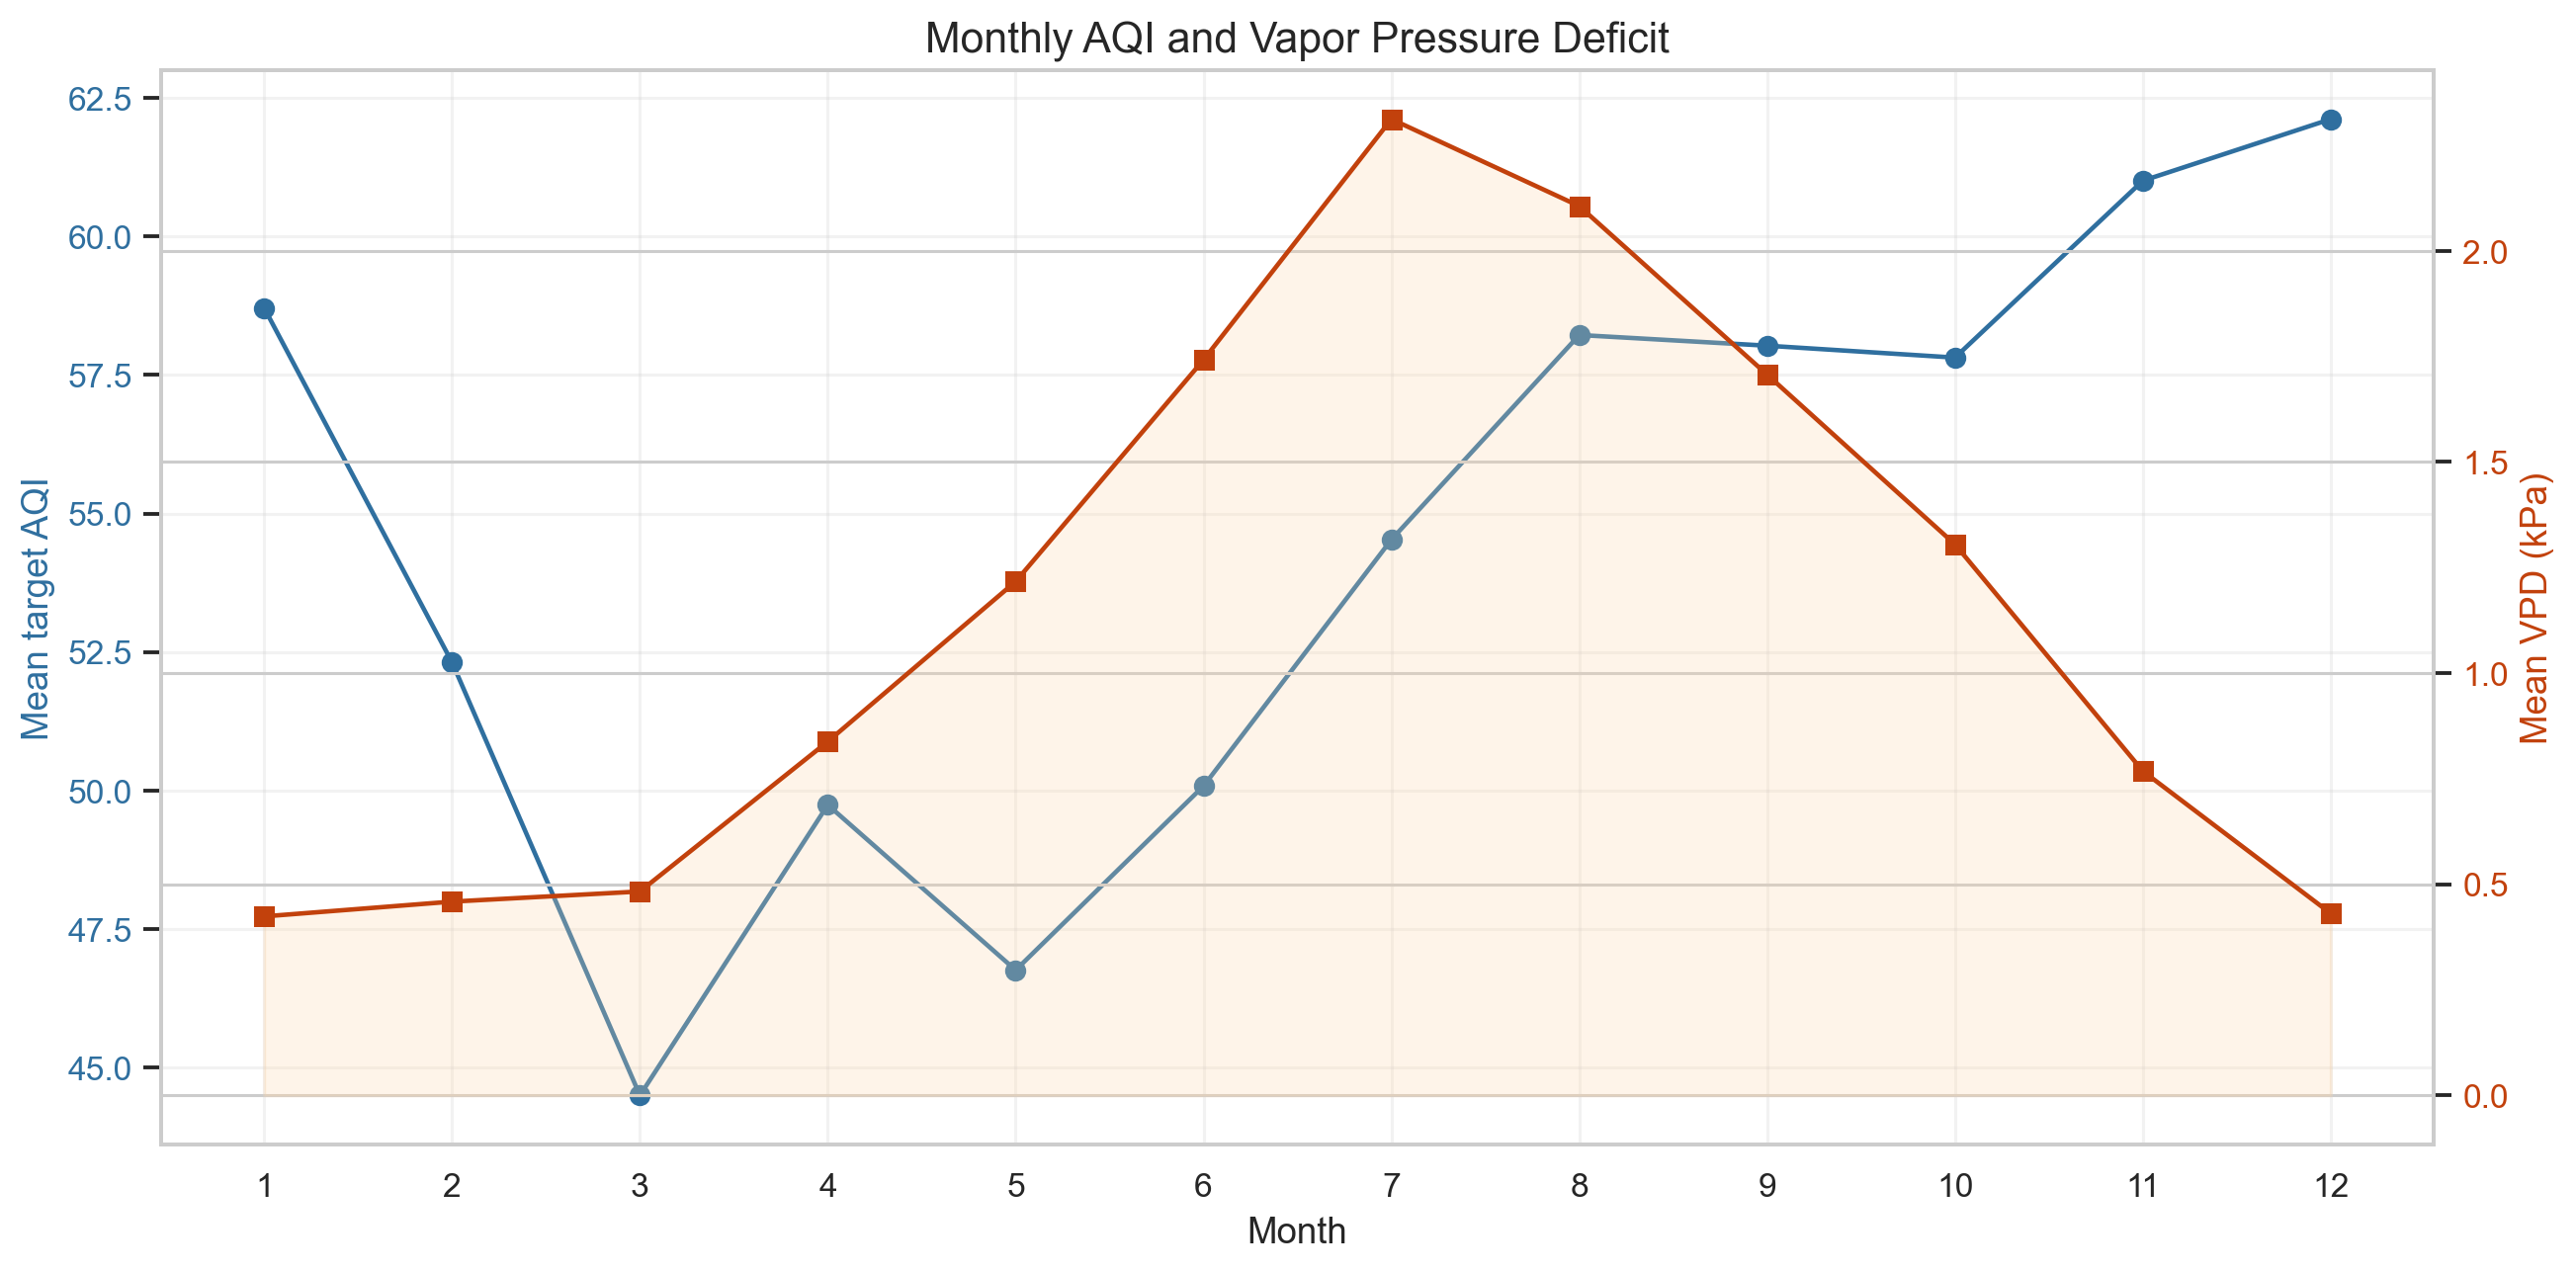
\includegraphics[width=0.74\linewidth]{data/plots/eda/07_vpd_monthly_diagnostic.png}
    \caption{Monthly diagnostic of recomputed VPD, used to inspect seasonal dryness structure in the AQI panel.}
    \label{fig:vpd-diagnostic}
\end{figure}
\FloatBarrier

\subsection{Temporal and Spatial Lag Features}
Temporal lag features encode recent and day-prior AQI states. For station $s$ at target time $t$, a local lag feature is represented as
\begin{equation}
    \mathrm{Lag}_{s,k}(t)=y_{s,t-k},
    \label{eq:local-lag}
\end{equation}
where $k$ is the lag horizon in hours. Spatial lag features summarize delayed AQI information from other stations or city-level sources:
\begin{equation}
    \mathrm{SpatialLag}_{s,k}(t)=
    \frac{1}{|\mathcal{N}(s)|}\sum_{j \in \mathcal{N}(s)} y_{j,t-k}.
    \label{eq:spatial-lag}
\end{equation}
These features are intended to provide transport-related context. Their value is tested empirically in the ablation study rather than assumed.

Additional engineered features include cyclic hour/month encodings, wind-vector decomposition, dry-heat interaction terms, dry-wind interaction terms, temperature-humidity ratios, and wind-speed-pressure ratios. Categorical station/source identifiers are retained for model families that can use categorical or one-hot encoded inputs.

\section{Methodology}
\subsection{Pipeline Overview}
The end-to-end workflow transforms raw monitoring and meteorological records into a leak-audited supervised learning benchmark. The pipeline includes data harmonization, feature engineering, chronological splitting, model training, leaderboard evaluation, scenario analysis, and ablation testing.

\begin{figure}[H]
    \centering
    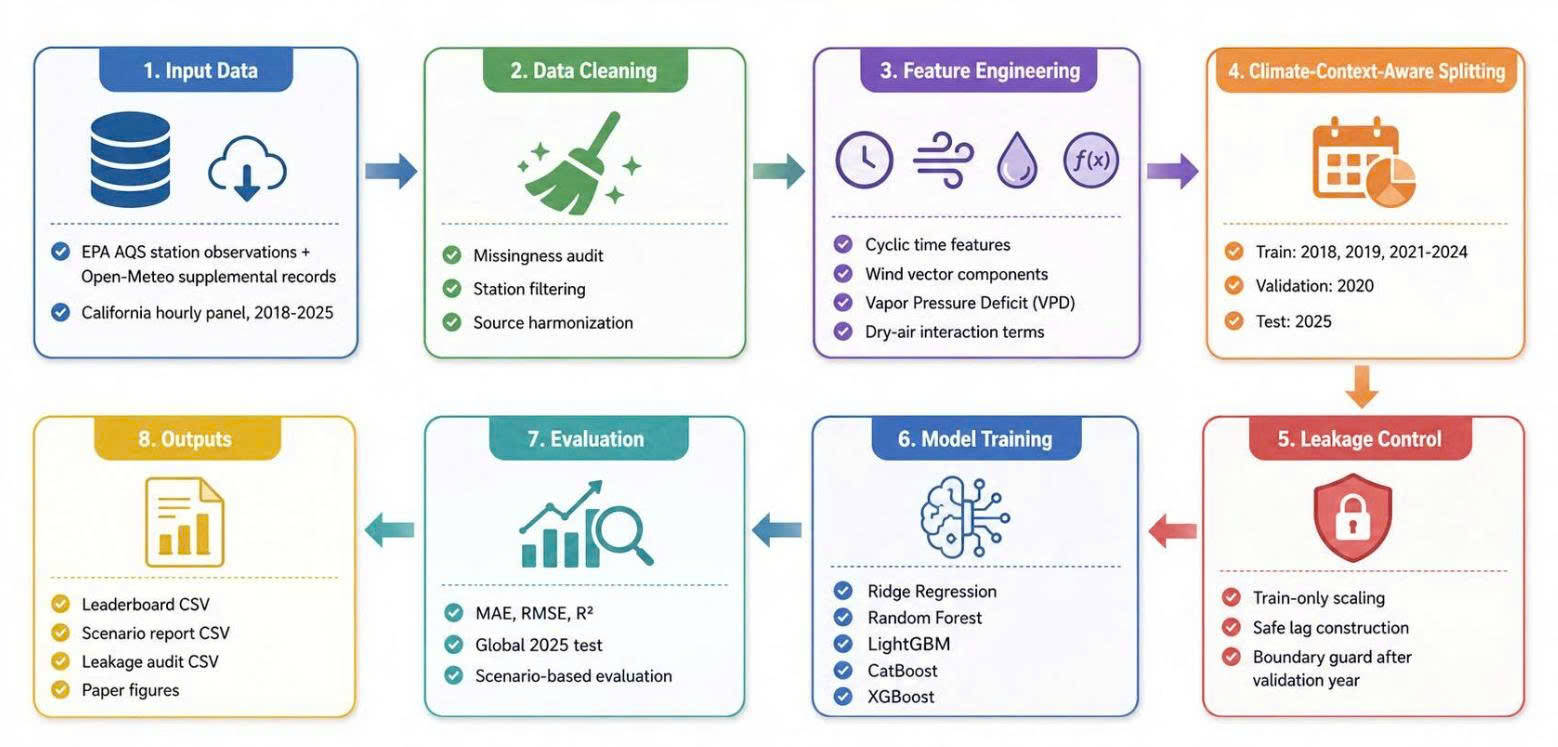
\includegraphics[width=0.82\linewidth]{data/plots/paper_workflow_pipeline_architecture.jpg}
    \caption{AQI forecasting pipeline architecture used in this study. The figure summarizes the conversion of EPA AQS and Open-Meteo records into leak-controlled training, validation, testing, and evaluation outputs.}
    \label{fig:pipeline-architecture}
\end{figure}
\FloatBarrier

\subsection{Forecasting Tasks}
For each station or source $s$ and target timestamp $t$, the supervised learning task is
\begin{equation}
    \hat{y}_{s,t+h}=f(\mathbf{x}_{s,t}),
    \label{eq:forecasting-task}
\end{equation}
where $\hat{y}_{s,t+h}$ is the predicted AQI, $h$ is the forecast horizon, and $\mathbf{x}_{s,t}$ contains meteorological variables, temporal encodings, categorical identifiers, engineered dryness features, lagged AQI features, and allowed spatial context.

Two configurations are evaluated. The short-term autoregressive setting predicts near-term AQI using recent local AQI lags from 1--3 hours. This setting is close to operational nowcasting and is expected to benefit strongly from temporal persistence. The long-term 24-hour setting predicts AQI one day ahead. It does not use local AQI from $t-1$ to $t-23$. The model must rely on weather, calendar structure, VPD, spatial lags, and day-prior or older local AQI information.

\subsection{Data Splitting Strategy}
The split is chronological and climate-context-aware rather than random. Random splitting is inappropriate for this problem because adjacent hourly observations share pollutant persistence, lag features, meteorological regimes, and station-specific seasonal structure. Mixing neighboring observations across train and test sets would overstate generalization.

\begin{table}[H]
\centering
\caption{Chronological data split used for model selection and final evaluation.}
\label{tab:data-split}
\begin{tabular}{>{\raggedright\arraybackslash}p{0.16\linewidth}
                >{\raggedright\arraybackslash}p{0.28\linewidth}
                >{\raggedright\arraybackslash}p{0.46\linewidth}}
\toprule
Partition & Years & Role and rationale \\
\midrule
Training & 2018, 2019, 2021--2024 & Fit model parameters using multiple non-test years. \\
Validation & 2020 & Tune and compare models on an extreme/wildfire-context year. \\
Test & 2025 & Final independent holdout year for reported performance. \\
\bottomrule
\end{tabular}
\end{table}
\FloatBarrier

The 2020 validation year is intentionally separated from training because it contains the highest concentration of extreme-AQI hours in the dataset and therefore provides a stress-oriented model-selection context. The 2025 test year is held out until final evaluation and is treated as the independent reporting year.

\subsection{Chronological Boundary Leakage Guard}
Because lagged features can cross partition boundaries, the pipeline applies a chronological boundary leakage guard. A record is allowed only when the temporal distance from a partition boundary is at least the scenario-specific guard:
\begin{equation}
    \Delta t_{\mathrm{boundary}} \geq G_h,
    \qquad
    G_h =
    \begin{cases}
    4 \text{ hours}, & \text{short-term nowcasting},\\
    215 \text{ hours}, & \text{long-term 24-hour forecasting}.
    \end{cases}
    \label{eq:boundary-guard}
\end{equation}
The leakage audit also confirms that future-like feature names and current PM2.5/PM10 proxy variables are absent from the model feature matrix.

\subsection{Models and Metrics}
Five models are evaluated: Linear Ridge, Random Forest, LightGBM, CatBoost, and XGBoost. Linear Ridge provides a regularized linear baseline. Random Forest represents bagging-based nonlinear learning. LightGBM, CatBoost, and XGBoost represent gradient-boosted decision-tree families. CatBoost receives categorical station/source identifiers natively; the other models use train-only preprocessing for categorical encoding and scaling where applicable.

Performance is reported with mean absolute error (MAE), root mean squared error (RMSE), and coefficient of determination ($R^2$):
\begin{equation}
    \mathrm{MAE}=\frac{1}{n}\sum_{i=1}^{n}|y_i-\hat{y}_i|,
    \label{eq:mae}
\end{equation}
\begin{equation}
    \mathrm{RMSE}=\sqrt{\frac{1}{n}\sum_{i=1}^{n}(y_i-\hat{y}_i)^2},
    \label{eq:rmse}
\end{equation}
\begin{equation}
    R^2=1-\frac{\sum_{i=1}^{n}(y_i-\hat{y}_i)^2}{\sum_{i=1}^{n}(y_i-\bar{y})^2}.
    \label{eq:r2}
\end{equation}

\section{Results and Discussion}
\subsection{Overall Leaderboard}
The 2025 test-year leaderboard shows a clear difference between near-term and 24-hour forecasting. Short-term nowcasting produces high $R^2$ values for all models, while 24-hour forecasting is substantially harder.

\subsection{Short-Term Nowcasting}
\begin{table}[H]
\centering
\caption{Short-term autoregressive nowcasting results on the 2025 test year.}
\label{tab:short-results}
\begin{tabular}{lrrr}
\toprule
Model & MAE & RMSE & $R^2$ \\
\midrule
LightGBM & 6.0716 & 9.5788 & 0.8691 \\
XGBoost & 5.8661 & 9.6352 & 0.8676 \\
Linear Ridge & 6.3330 & 9.7258 & 0.8651 \\
CatBoost & 6.2556 & 10.0873 & 0.8549 \\
Random Forest & 6.6096 & 10.1534 & 0.8530 \\
\bottomrule
\end{tabular}
\end{table}
\FloatBarrier

LightGBM obtains the highest short-term $R^2$ at 0.8691, while XGBoost obtains the lowest MAE. All models exceed 0.85 in $R^2$, indicating that recent AQI history is highly informative for near-term nowcasting. This result should be interpreted as evidence of strong temporal persistence rather than as evidence that the models fully understand atmospheric mechanisms. The leakage audit reports a 0.927 correlation between the 2025 target and the one-hour AQI lag, which explains why even Linear Ridge remains competitive.

\subsection{Long-Term 24-Hour Forecasting}
\begin{table}[H]
\centering
\caption{Long-term 24-hour forecasting results on the 2025 test year.}
\label{tab:long-results}
\begin{tabular}{lrrr}
\toprule
Model & MAE & RMSE & $R^2$ \\
\midrule
LightGBM & 13.5546 & 19.4498 & 0.4605 \\
Linear Ridge & 13.5542 & 19.4738 & 0.4592 \\
XGBoost & 13.6759 & 19.5251 & 0.4563 \\
CatBoost & 13.6208 & 20.3258 & 0.4108 \\
Random Forest & 14.2465 & 20.6329 & 0.3929 \\
\bottomrule
\end{tabular}
\end{table}
\FloatBarrier

The long-term task is harder because local AQI observations from $t-1$ to $t-23$ are excluded. LightGBM again achieves the highest $R^2$, but its advantage over Linear Ridge and XGBoost is small. This suggests that 24-hour AQI prediction depends on smoother day-prior structure, seasonal timing, and meteorological context, while abrupt upper-tail events remain difficult to anticipate from the available tabular features alone.

\subsection{Extreme-Event and Climate-Context Interpretation}
Global test-year metrics do not fully describe operational forecasting risk because AQI errors are not equally important across health categories and climate contexts. Fig.~\ref{fig:aqi-category-timeline} therefore provides an EDA view of the daily AQI trajectory colored by U.S. AQI category. Most daily observations fall in the Good and Moderate ranges, but the figure also shows episodic transitions into Unhealthy, Very Unhealthy, and occasional Hazardous conditions. These intermittent upper-tail periods motivate scenario-specific reporting alongside the global leaderboard.

\begin{figure}[H]
    \centering
    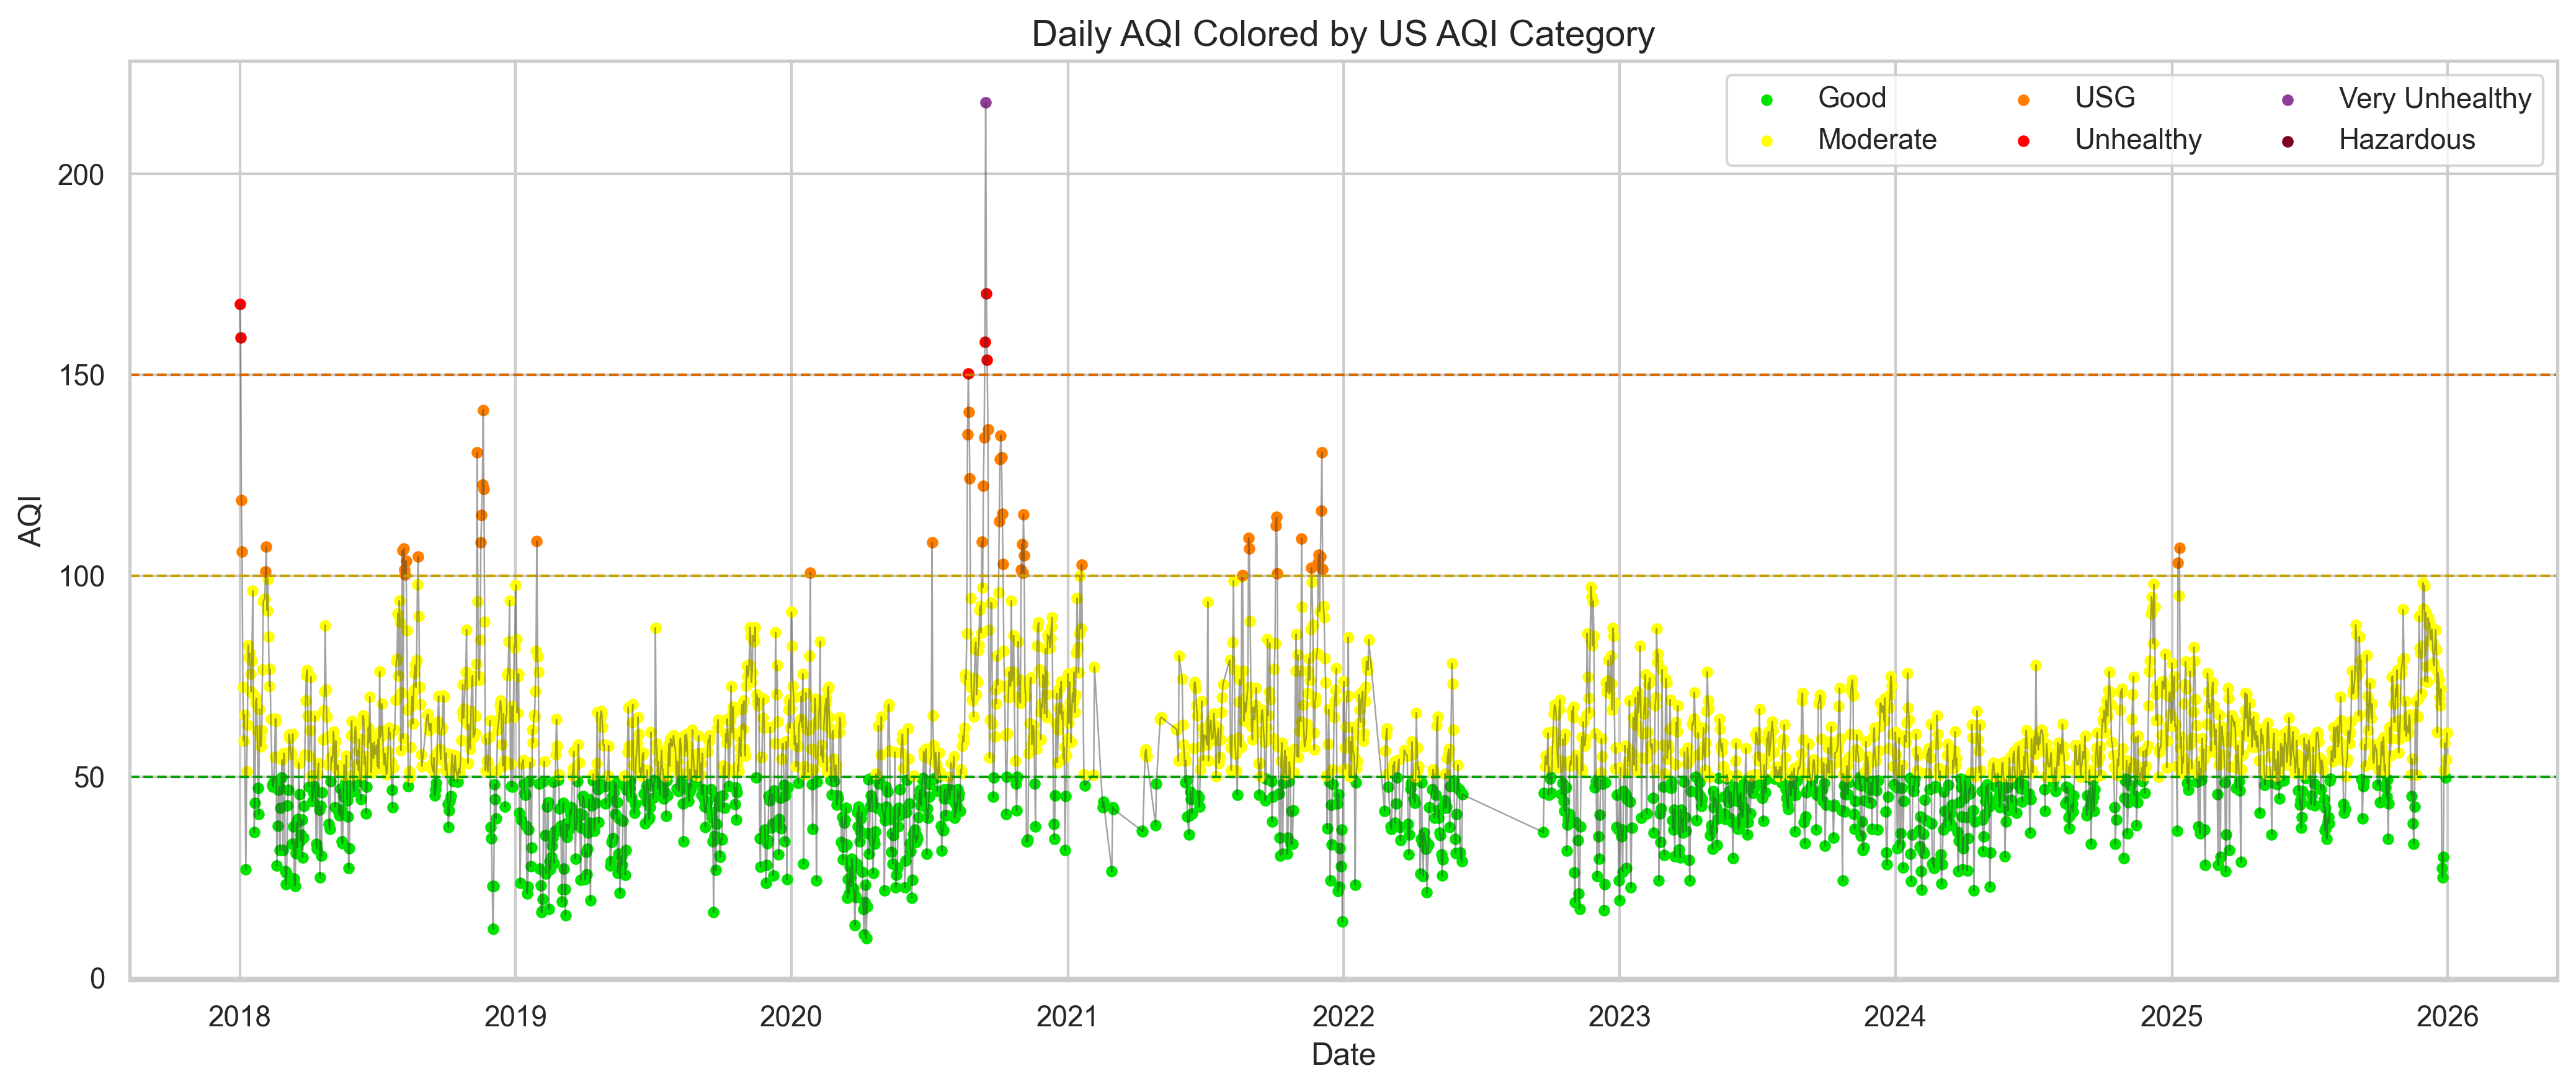
\includegraphics[width=0.88\linewidth]{data/plots/eda_aqi_category_timeline.png}
    \caption{Daily AQI observations colored by U.S. AQI health category. The category-colored timeline illustrates the dominance of Good and Moderate days while highlighting episodic high-AQI periods that motivate scenario-level and extreme-event evaluation.}
    \label{fig:aqi-category-timeline}
\end{figure}
\FloatBarrier

Table~\ref{tab:scenario-context-results} reports the best model for each scenario slice, where ``best'' is selected by $R^2$ within the same forecasting configuration and scenario. The climate-context interpretation separates ordinary low-to-moderate AQI behavior from stress windows and upper-tail events. The January slice is reported as the January 2025 Winter Extreme-AQI Window, rather than as a causal wildfire label, because the model-ready dataset does not include verified fire perimeter, smoke plume, or satellite aerosol features.

\begin{table}[H]
\centering
\caption{Best-per-scenario results for extreme-event and climate-context evaluation on the 2025 test year.}
\label{tab:scenario-context-results}
\footnotesize
\setlength{\tabcolsep}{3pt}
\resizebox{\textwidth}{!}{%
\begin{tabular}{lllrrrr}
\toprule
Configuration & Scenario slice & Best model & $N$ & MAE & RMSE & $R^2$ \\
\midrule
Short-term & Full 2025 test year & LightGBM & 26297 & 6.0716 & 9.5788 & 0.8691 \\
Short-term & Non-event baseline (AQI $\leq 100$) & XGBoost & 24806 & 5.1896 & 7.4627 & 0.8514 \\
Short-term & January 2025 Winter Extreme-AQI Window & Linear Ridge & 1799 & 9.3585 & 14.8151 & 0.8430 \\
Short-term & Extreme AQI in 2025 (top 5\%) & Linear Ridge & 1325 & 19.4746 & 25.6386 & 0.1715 \\
Short-term & July--September 2025 wildfire season & Linear Ridge & 6624 & 6.1250 & 10.2926 & 0.8539 \\
Long-term & Full 2025 test year & LightGBM & 26297 & 13.5546 & 19.4498 & 0.4605 \\
Long-term & Non-event baseline (AQI $\leq 100$) & CatBoost & 24806 & 11.2581 & 14.6878 & 0.4242 \\
Long-term & January 2025 Winter Extreme-AQI Window & LightGBM & 1799 & 19.9117 & 32.8818 & 0.2265 \\
Long-term & Extreme AQI in 2025 (top 5\%) & LightGBM & 1325 & 45.6488 & 54.8257 & -2.7887 \\
Long-term & July--September 2025 wildfire season & Linear Ridge & 6624 & 13.1165 & 18.9501 & 0.5047 \\
\bottomrule
\end{tabular}%
}
\end{table}
\FloatBarrier

The table clarifies three patterns. First, short-term nowcasting remains strong for the full year, the non-event baseline, the January winter window, and the July--September seasonal slice because recent AQI persistence is still available. Second, the top-5\% AQI slice is much harder even in the short-term setting, with the best $R^2$ falling to 0.1715. Third, the 24-hour top-tail scenario produces negative $R^2$, meaning that the selected model performs worse than a scenario-specific mean predictor on this restricted subset. This does not contradict the global leaderboard; rather, it shows that rare upper-tail AQI behavior is not sufficiently represented by weather, VPD, spatial lags, and day-prior AQI alone.

\subsection{Prediction Diagnostics}
The predicted-versus-actual diagnostic for LightGBM confirms the main quantitative pattern. The model tracks central AQI ranges well, especially in the short-term setting, but high-AQI peaks are more dispersed and harder to reproduce accurately. This supports the need for explicit extreme-event analysis and for future event-aware features.

\begin{figure}[H]
    \centering
    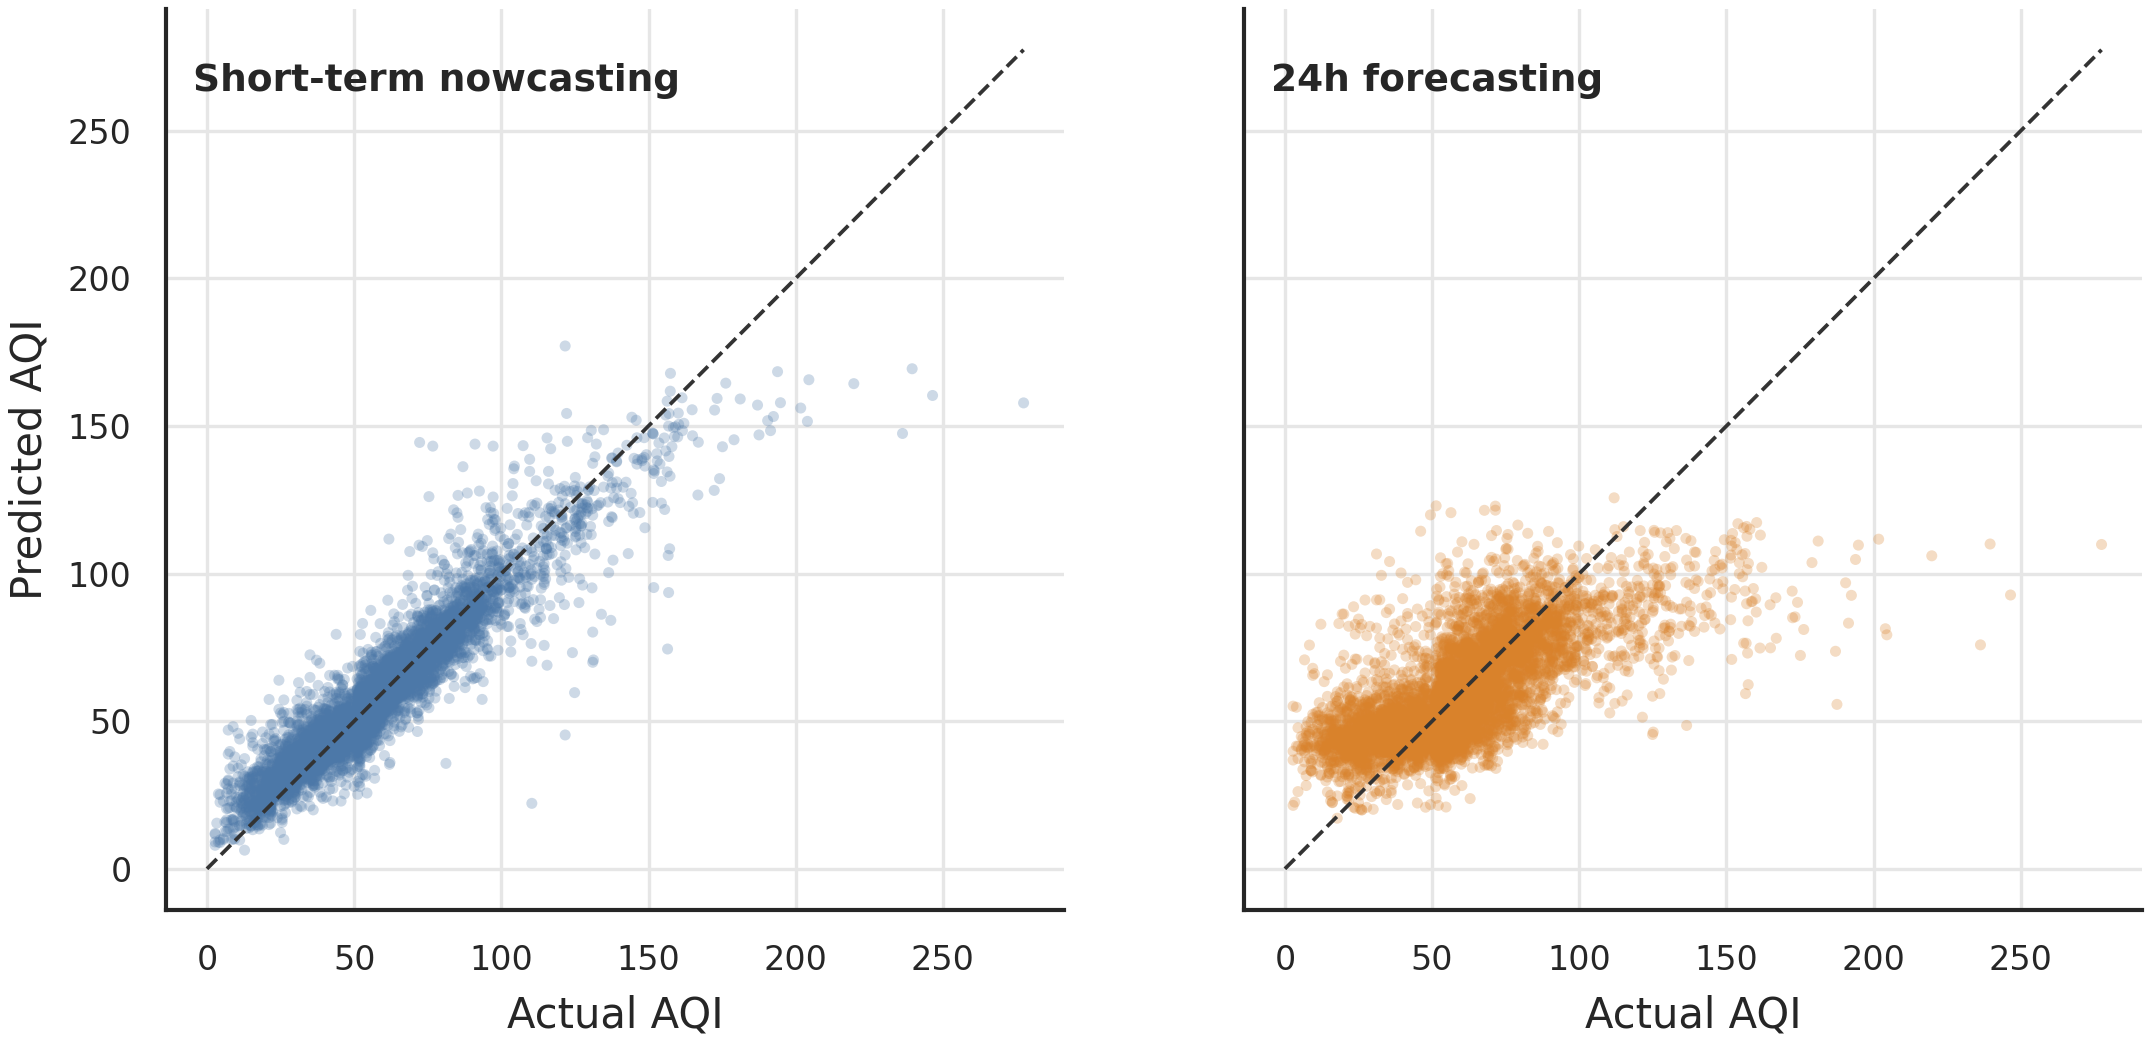
\includegraphics[width=0.78\linewidth]{data/plots/paper_lightgbm_predicted_vs_actual.png}
    \caption{Predicted versus actual AQI for LightGBM on the independent 2025 test year.}
    \label{fig:lightgbm-predicted-actual}
\end{figure}
\FloatBarrier

\section{Ablation Study}
A focused LightGBM ablation study tests whether VPD and spatial lag features provide measurable standalone gains. The full feature set is compared with two variants: one removing only VPD, and one removing all spatial lag features. Delta columns are computed relative to the full LightGBM model within the same forecasting configuration.

\begin{table}[H]
\centering
\caption{LightGBM ablation study for VPD and spatial lag features on the 2025 test year.}
\label{tab:ablation}
\resizebox{\textwidth}{!}{%
\begin{tabular}{llrrrrrr}
\toprule
Configuration & Feature set & Features & MAE & RMSE & $R^2$ & $\Delta$MAE & $\Delta R^2$ \\
\midrule
Short-term & Full feature set & 47 & 6.0716 & 9.5788 & 0.8691 & -- & -- \\
Short-term & Without VPD & 46 & 6.0772 & 9.5953 & 0.8687 & 0.0056 & -0.0005 \\
Short-term & Without spatial lags & 32 & 6.0558 & 9.4794 & 0.8718 & -0.0158 & 0.0027 \\
Long-term & Full feature set & 62 & 13.5546 & 19.4498 & 0.4605 & -- & -- \\
Long-term & Without VPD & 61 & 13.5309 & 19.4410 & 0.4610 & -0.0237 & 0.0005 \\
Long-term & Without spatial lags & 37 & 13.6660 & 19.4500 & 0.4605 & 0.1114 & 0.0000 \\
\bottomrule
\end{tabular}%
}
\end{table}
\FloatBarrier

The ablation results do not support a strong independent VPD performance claim. Removing VPD changes $R^2$ by less than 0.001 in both configurations, and the direction of the change is not consistently favorable to the full feature set. Therefore, VPD should be described as an engineered dryness feature rather than as a demonstrated accuracy-improving feature.

The spatial-lag result is also mixed. Removing spatial lags slightly improves short-term $R^2$, which is plausible because short-term nowcasting is already dominated by local AQI persistence from the 1--3 hour lags. In the long-term setting, removing spatial lags increases MAE by 0.1114 but leaves $R^2$ almost unchanged. This suggests a modest long-horizon error-reduction role, but not a large explained-variance gain.

\section{Extreme-Event Analysis}
Extreme AQI hours are defined using the empirical 99th percentile of the full model-ready target distribution. The threshold is
\begin{equation}
    y_t > P_{99} = 151.84.
    \label{eq:extreme-threshold}
\end{equation}
Using this definition, the dataset contains 1,802 extreme hourly records, approximately 0.99\% of all observations. The year 2020 contains the largest number of extreme hours, and August--October accounts for approximately 42.8\% of all extreme records.

\begin{figure}[H]
    \centering
    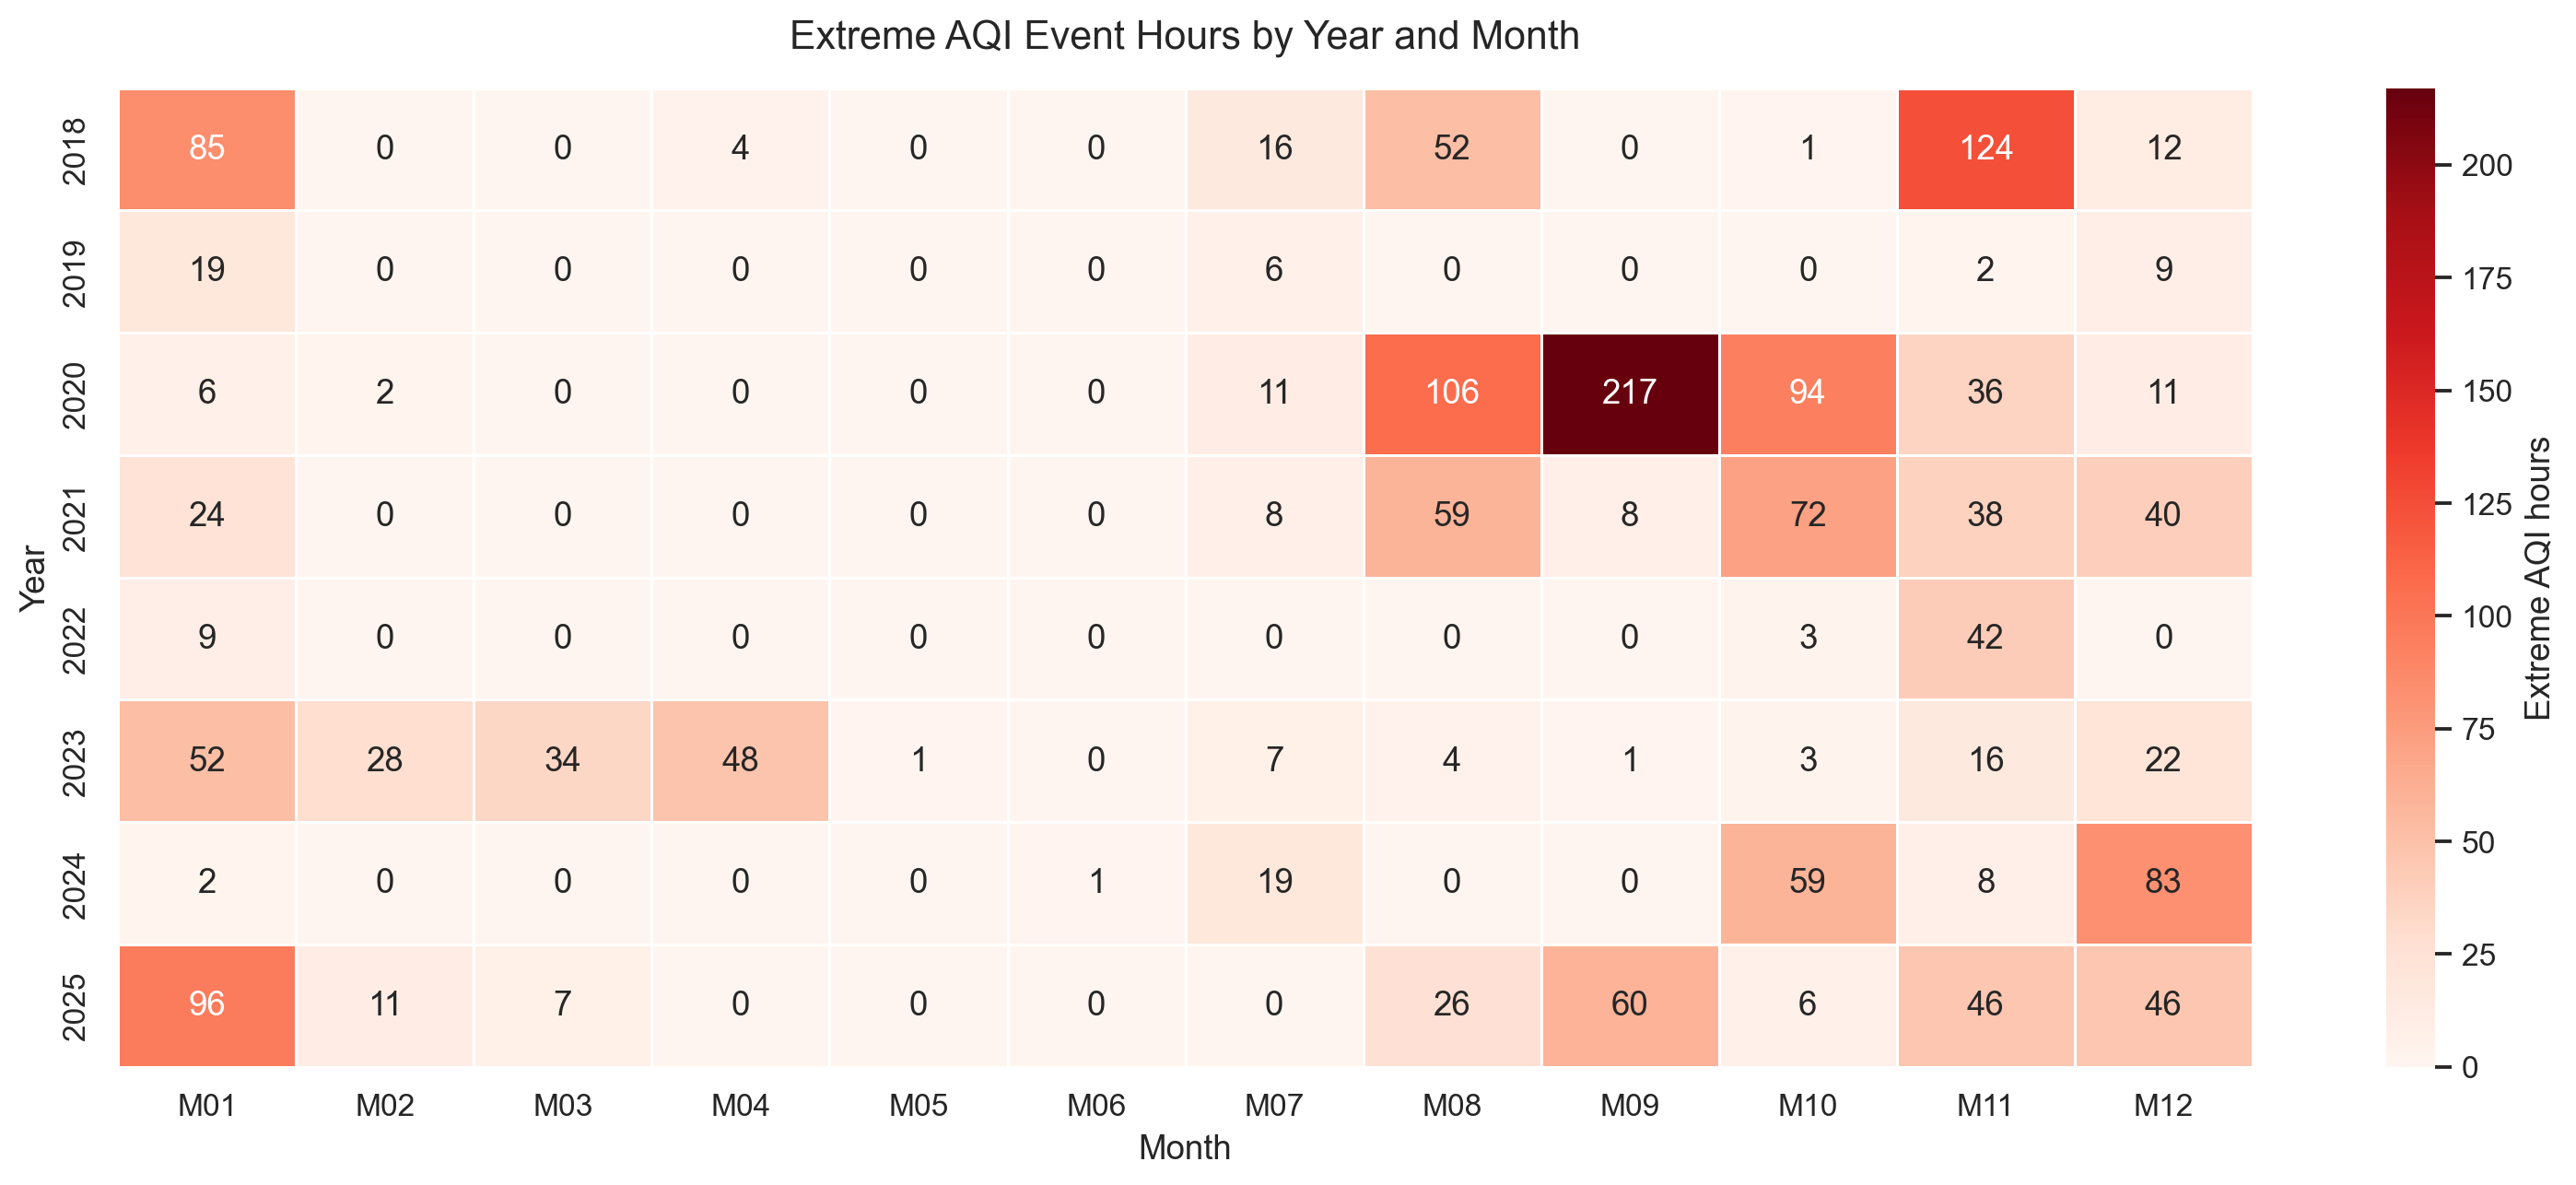
\includegraphics[width=0.74\linewidth]{data/plots/eda/06_extreme_aqi_events_heatmap_year_month.png}
    \caption{Year-month heatmap of extreme AQI records defined by the empirical 99th percentile threshold.}
    \label{fig:extreme-heatmap}
\end{figure}
\FloatBarrier

The heatmap indicates temporal clustering rather than uniform random occurrence. The concentration in 2020 and in late-summer to autumn months is consistent with a wildfire-season context, but this paper does not make causal wildfire attribution. Establishing causality would require joining the AQI panel with external fire perimeters, smoke plume trajectories, aerosol optical depth, wind transport, or satellite-based smoke products.

\section{Threats to Validity}
Several limitations should be considered when interpreting the results. First, \texttt{target\_aqi} is a PM2.5-derived AQI proxy, not a complete regulatory AQI label derived from all criteria pollutants. Second, the dataset combines EPA station observations with Open-Meteo supplemental records, which may introduce source heterogeneity. Third, the 2025 test-year distribution is affected by the available supplemental sources after temporal alignment, so station-level generalization should be interpreted carefully. Fourth, VPD and spatial lags are physically motivated engineered features, but the ablation study shows limited standalone evidence of improvement. Fifth, the extreme-event section identifies temporal clustering only; without external fire and smoke observations, it cannot attribute high-AQI records to wildfire causes.

\section{Conclusion and Future Work}
This paper presented a California US AQI forecasting benchmark with climate-context and extreme-event evaluation. Using 181,122 hourly observations from 2018--2025, the study compared Linear Ridge, Random Forest, LightGBM, CatBoost, and XGBoost under short-term nowcasting and 24-hour forecasting scenarios. LightGBM achieved the best $R^2$ in both settings, with 0.8691 for short-term nowcasting and 0.4605 for long-term forecasting.

The results show that near-term AQI prediction is strongly driven by temporal persistence, while 24-hour and upper-tail AQI forecasting remain difficult when recent local AQI is hidden. The VPD ablation result is especially important for academic wording: VPD is best described as an engineered dryness feature, not as a proven standalone performance driver. Spatial lags provide mixed evidence, with at most modest long-term MAE benefit. Future work should integrate event-aware data such as fire perimeters, smoke plumes, aerosol optical depth, planetary boundary-layer height, and upwind transport indicators. It should also extend ablation testing across model families and feature groups, and evaluate uncertainty-aware warning thresholds for high-AQI conditions.

\begingroup
\small
\bibliographystyle{IEEEtran}
\bibliography{references}
\endgroup

\end{document}
